\documentclass{beamer}
%
% Choose how your presentation looks.
%
% For more themes, color themes and font themes, see:
% http://deic.uab.es/~iblanes/beamer_gallery/index_by_theme.html
%
\mode<presentation>
{
  \usetheme{default}      % or try Darmstadt, Madrid, Warsaw, ...
  \usecolortheme{default} % or try albatross, beaver, crane, ...
  \usefonttheme{default}  % or try serif, structurebold, ...
  \setbeamertemplate{navigation symbols}{}
  \setbeamertemplate{caption}[numbered]
} 

\usepackage[english]{babel}
\usepackage[utf8]{inputenc}
\usepackage[T1]{fontenc}
\usepackage{xcolor}
\usepackage{listings}
\usepackage{graphicx}
\usepackage{ stmaryrd }

\lstset{
  basicstyle=\ttfamily\small, % Style de base pour le code
  keywordstyle=\color{blue},  % Couleur des mots-clés
  commentstyle=\color{gray},  % Couleur des commentaires
  stringstyle=\color{red},    % Couleur des chaînes de caractères
  showstringspaces=false,     % Ne pas montrer les espaces dans les chaînes
  numbers=left,               % Numérotation des lignes sur la gauche
  numberstyle=\tiny\color{gray}, % Style de la numérotation des lignes
  stepnumber=1,               % Numérotation des lignes à chaque ligne
  frame=single,               % Encadrer le code
  breaklines=true,            % Casser les lignes trop longues
  captionpos=b,               % Position de la légende en bas
  tabsize=4                   % Taille des tabulations
}

\title[Your Short Title]{Représentation Numérique}
\subtitle{Skew Binary Numbers}
\author{Crague Ilian, supervision de Pierre-Evariste Dagand}
\institute{IRIF}

\begin{document}

\begin{frame}
  \titlepage
\end{frame}

% Uncomment these lines for an automatically generated outline.
%\begin{frame}{Outline}
%  \tableofcontents
%\end{frame}

\section{Introduction}
\newcommand{\denote}[1]{\ensuremath{\llbracket #1 \rrbracket}}
\newcommand{\aSbin}[1][0]{\ensuremath{\alpha}}
\newcommand{\aDigit}[1][i]{\ensuremath{a_{#1}}}
\begin{frame}{Definition}

\begin{block}{Skew Binary Number}

  Let $ \aSbin = \aDigit[n] \aDigit[n-1] \ldots \aDigit[1]$ be a skew binary number with $\aDigit \in \{0, 1, 2\}$.
  
  We define:
  $$\denote{\aSbin} \triangleq \sum_{i = 1}^{n} \aDigit[i] (2^{i} - 1)$$
\end{block}


\begin{block}{Example}
\begin{align*}
    \denote{210} &= 0 \cdot (2^{1} - 1) + 1 \cdot (2^{2} - 1) + 2 \cdot (2^{3} - 1)\\
    &= 17_{10}\\
    \denote{1002} &= 1 \cdot (2^1 - 1) + 2 \cdot (2^4 - 1)\\
    &=17_{10}
\end{align*} 
\end{block}
\end{frame}


\begin{itemize}
\item Théorème : Tout entier naturel admet une représentation en \textit{skew bin}
\end{itemize}



\begin{frame}{Canonicity}
\begin{block}{Proposition: canonicity}
Every skew binary admits a unique representation of the form
$$(1 \mid 0)^* (20^*)^?$$
\end{block}

\begin{block}{Example}
\begin{align*}
    17_{10} &= 2_{10} + (2^4 - 1)\\
    &= 2 \cdot (2^1 - 1) + (2^4 - 1)\\
    &= \denote{20} + \denote{1000}\\
    &= \denote{1020}
\end{align*}  
\end{block}

\end{frame}


\begin{frame}{Introduction : Pourquoi ?}

 
Soit $\alpha$ un \textit{SBin} sous forme canonique, $\alpha + 1$ ?
\begin{itemize}
    \item Si le plus petit coefficient non nul est 2 :\\
    On remarque : $1 + 2 \cdot (2^i -1) = 2^{i + 1} - 1$\\
    On passe ce coefficient à 0 et on incrémente le cofficient suivant.
    \item Si le plus petit coefficient non nul est 1 :\\
    On incrémente le bit de poids faible.
\end{itemize}

$\rightarrow$ L'incrément des \textit{skew bin} est en temps constant ( O(1) ).\\
$\rightarrow$L'ensemble des \textit{skew bin} en forme canonique est clos par incrément.


\begin{block}{Exemples}

$ [102] = 9, \phantom{.} \bullet102 + \bullet 1 = \bullet 110, \phantom{.} [110] = 10 $
$ [12] = 5, \phantom{.} \bullet 12 + \bullet 1 = \bullet 20, \phantom{.} [20] = 6$
$ [101] = 8, \phantom{.} \bullet101 + \bullet1 = \bullet 102, \phantom{.} [102] = 9 $
$ [110] = 10, \phantom{.} \bullet110 + \bullet1 = \bullet111, \phantom{.} [111] = 11 $
\end{block}

\end{frame}

\begin{frame}{Que peut-on faire avec les \textit{skew bin} ?}

\begin{itemize}
    \item inc : $\alpha \rightarrow \alpha + 1$
    \item dec : $\alpha \rightarrow \alpha - 1$,  même idée que inc, temps constant ( 0(1) )
    \item is\_canonical : $\alpha \rightarrow bool$
    \item skew\_to\_int : $\alpha \rightarrow [\alpha]$
    \item skew\_from\_int : $[\alpha] \rightarrow \alpha$ (grâce à l'existence et l'unicité)
    
\end{itemize}

\vskip 1cm

\begin{center}
    Choix : représenter nos \textit{skew bin} sous cette forme :
$ ...^{d_1} a_1 ...\phantom{.} ...^{d_{n-1}} a_{n-1} \phantom{.}...^{d_n} a_n $\\
Par exemple :
$ \bullet 1020 : (T, 1) :: (O, 1) :: []$
\end{center}


\end{frame}

\begin{frame}[fragile]{Skew bin : is\_canonical}
\begin{lstlisting}
let is_canonical : skew -> bool = function
  | (T, n) :: rest ->
      n >= 0 && List.for_all (fun (w, n) -> w = O && n >= 0) rest
  | l -> List.for_all (fun (w, n) -> w = O && n >= 0) l
\end{lstlisting}
\end{frame}

\begin{frame}[fragile]{Skew bin : inc}
\begin{lstlisting}
let inc s =
  assert (is_canonical s);
  match s with
  | [] -> (O, 0) :: []
  | (T, n) :: [] -> (O, n + 1) :: []
  | (O, n) :: [] -> if n = 0 then (T, n) :: [] 
                    else [ (O, 0); (O, n - 1) ]
  | (O, 0) :: (O, n2) :: rest -> 
        (T, 0) :: (O, n2) :: rest
  | (O, n1) :: (O, n2) :: rest -> 
        (O, 0) :: (O, n1 - 1) :: (O, n2) :: rest
  | (T, n1) :: (O, 0) :: rest -> (T, n1 + 1) :: rest
  | (T, n1) :: (O, n2) :: rest -> 
        (O, n1 + 1) :: (O, n2 - 1) :: rest
  | _ -> assert false
\end{lstlisting}
\end{frame}


\begin{frame}[fragile]{Skew bin : dec}
\begin{lstlisting}
let dec s =
  let plus_1 = function [] -> [] | (a, n) :: rest -> (a, n + 1) :: rest in
  assert (is_canonical s);
  match s with
  | [] -> raise (Failure "sub_1")
  | (O, 0) :: rest -> plus_1 rest
  | (O, n) :: rest -> (T, n - 1) :: plus_1 rest
  | (T, 0) :: rest -> (O, 0) :: rest
  | (T, n) :: rest -> (T, n - 1) :: (O, 0) :: rest
\end{lstlisting}
On utilise l'égalité suivante :
$2 \cdot (2^i -1) - 1 = 2 \cdot (2^{i - 1} - 1) + (2^{i} - 1)$

\end{frame}

\begin{frame}[fragile]{Skew bin : skew\_to\_int}
\begin{lstlisting}
let skew_to_int s =
  let rec aux s acc pow =
    match s with
    | [] -> 0
    | (d, n) :: rest ->
        let w = if d = O then 1 else 2 in
        let new_acc = acc + pow in
        let next_pow = 2 * pow in
        if n = 0 then (w * acc) + aux rest new_acc next_pow
        else aux ((d, n - 1) :: rest) new_acc next_pow
  in
  assert (is_canonical s);
  aux s 1 2
\end{lstlisting}
\end{frame}

\begin{frame}[fragile]{Skew bin : skew\_from\_int}
\begin{lstlisting}
let skew_from_int n =
  (*returns (k, pow) with the greatest pow < n, pow 2^{k+1} - 1*) 
  let greatest_pow k pow n =
    ...
  in
  let rec aux n =
    if n = 0 then []
    else
      let k, pow = greatest_pow 0 2 n in
      if n = 2 * pow then (T, k) :: [] else (O, k) :: aux (n - pow)
  in
  aux n
\end{lstlisting}
\end{frame}

\begin{frame}{Skew bin}
    Ok c'est bien... Mais après ?\\
    \phantom{Les Skew Random Access List (Skew RAL, ou RAL)}
    
\end{frame}

\begin{frame}{Skew bin}
    Ok c'est bien... Mais après ?\\
    Les Skew Random Access List (Skew RAL, ou RAL)
    
\end{frame}


\begin{frame}[fragile]{Skew RAL}
\begin{columns}

    \begin{column}{0.6\textwidth}

    On remarque que $2^{n+1} - 1$ est la taille d'un arbre binaire complet de profondeur $n$ :\\
    $\sum_{i = 0}^{n} 2^{i} = 2^0 \cdot \frac{1 - 2^{n + 1}}{1 - 2} = 2^{n+1} - 1$\\
    \vskip 0.3 cm
    On décore chaque coefficient de notre \textit{skew bin} avec un arbre de la bonne taille
    \end{column}
    
    \begin{column}{0.3\textwidth}

\begin{figure}
    \centering
   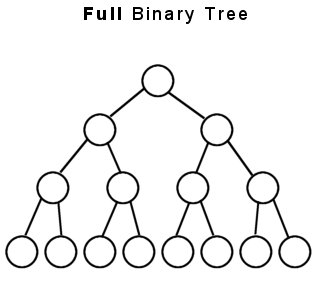
\includegraphics[width=\textwidth]{FullBinary-3822745123.jpg}
\end{figure}
        
\end{column}
\end{columns}

\end{frame}

\begin{frame}{Skew RAL}
Par exemple, le \textit{Skew bin} $\bullet 1020$ devient : \\
    \begin{figure}
    \centering
   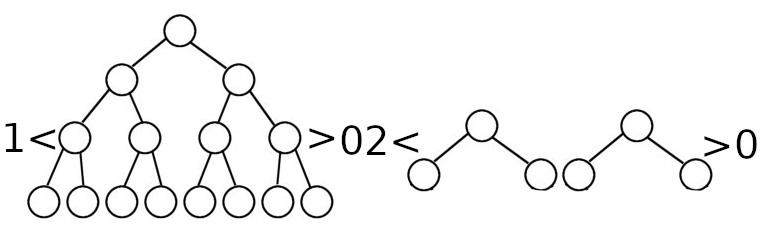
\includegraphics[width=\textwidth]{exemple_ral.png}
\end{figure}

Nous allons maintenant chercher à définir des opérations sur les RAL de manière à avoir une équivalence entre \textit{RAL} et les \textit{list OCaml}.
\end{frame}

\begin{frame}[fragile]{Skew RAL : Choix d'implémentation}
Nous avons choisi d'adapter l'implémentation d'Okasaki pour les RAL à notre implémentation des skew bin.

\begin{lstlisting}
type 'a array_digit =
  | One of (int * 'a tree)
  | Two of (int * 'a tree * 'a tree)
type 'a ral = (int * 'a array_digit) list
\end{lstlisting}

Différences avec l'implémentation d'Okasaki :
\begin{itemize}
    \item Nous ne stockons pas les $0$
    \item Nous considérons les $2$ comme un élément à par entière, lui considère un $2$ comme deux $1$
\end{itemize}

    
\end{frame}

\begin{frame}{Skew RAL}
\begin{itemize}
    \item to\_bin : $'a$ RAL $\rightarrow$ SBin
    \item is\_well\_formed : $'a$ RAL $\rightarrow$ bool
    \item cons : $'a$ $\rightarrow$ $'a$ RAL $\rightarrow$ $'a$ RAL
    \item head : $'a$ RAL $\rightarrow$ $'a$
    \item tail : $'a$ RAL $\rightarrow$ $'a$ RAL
    \item  to\_list : $'a$ RAL $\rightarrow$ $'a$ $list$
    \item from\_list : $'a$ $list$ $\rightarrow$ $'a$ RAL
    \item lookup : $int$ $\rightarrow$ $'a$ RAL $\rightarrow$ $'a$
    \item update : $'a$ $\rightarrow$ $int$ $\rightarrow$ $'a$ RAL $\rightarrow$ $'a$
\end{itemize}

    
\end{frame}

\begin{frame}{Skew RAL}
\begin{itemize}
    \item to\_bin : RAL $\rightarrow$ SBin\\ On enlève les arbres
    \item is\_well\_formed : RAL $\rightarrow$ bool\\ On vérifie que le to\_bin du RAL est canonique et que chaque arbre a la bonne taille
    \item  cons : $'a$ $\rightarrow$ $'a$ RAL $\rightarrow$ $'a$ RAL\\cons est construit sur la base de inc
    \item tail : $'a$ RAL $\rightarrow$ $'a$ RAL\\tail est construit sur la base de dec
\end{itemize}
cons, head, tail et lookup sont construits de manière à ce qu'ils soient équivalents à leurs homologues des $list$ $OCaml$
\end{frame}

\begin{frame}[fragile]{Skew RAL : is\_well\_formed}
    \begin{lstlisting}
let is_well_formed s =
  let rec aux s acc =
    match s with
    | [] -> true
    | (w, One (n, t)) :: rest ->
        let new_acc = 2 * acc in
        if n = 0 then w = card t && card t = acc - 1 && aux rest new_acc
        else aux ((w, One (n - 1, t)) :: rest) new_acc
    | _ -> false
  in
  match s with
  | [] -> true
  | (_, One (_, _)) :: _ -> aux s 2
  | (w, Two (n, t1, t2)) :: rest ->
      w = card t1 && card t1 = card t2 && card t1 = pow_2 (n + 1) - 1
      && let acc = pow_2 (n + 2) in aux rest acc
\end{lstlisting}
\end{frame}

\begin{frame}[fragile]{Skew RAL : cons}
\begin{lstlisting}
let cons x st =
  assert (is_well_formed st);
  match st with
  | [] -> (1, One (0, Leaf x)) :: []
  | (w, Two (n, t1, t2)) :: [] ->
      ((2 * (w + 1)) - 1, One (n + 1, Node (x, t1, t2))) :: []
  | (w, One (0, t)) :: [] -> (w, Two (0, t, Leaf x)) :: []
  | (w, One (n, t)) :: [] -> [ (1, One (0, Leaf x)); (w, One (n - 1, t)) ]
 ...
\end{lstlisting}
\end{frame}

\begin{frame}[fragile]{Skew RAL : tail}
\begin{lstlisting}
let tail st =
  let plus_1 = function
    | [] -> []
    | (w, One (n, t)) :: rest -> (w, One (n + 1, t)) :: rest
    | (w, Two (n, t1, t2)) :: rest -> (w, Two (n + 1, t1, t2)) :: rest
  in
  assert (is_well_formed st);
  match st with
  | [] -> raise (Failure "tail")
  | (1, One (0, Leaf _)) :: rest -> plus_1 rest
  | (w, One (n, Node (_, t1, t2))) :: rest ->
      (w / 2, Two (n - 1, t1, t2)) :: plus_1 rest
  | (1, Two (0, Leaf t1, Leaf _)) :: rest -> (1, One (0, Leaf t1)) :: rest
  ...
\end{lstlisting}    
\end{frame}

\begin{frame}[fragile]{Skew RAL : head}
\begin{lstlisting}
let head st =
  assert (is_well_formed st);
  match st with
  | [] -> raise (Failure "head")
  | (1, One (0, Leaf a)) :: _ -> a
  | (_, One (_, Node (a, _, _))) :: _ -> a
  | (1, Two (0, Leaf _, Leaf a)) :: _ -> a
  | (_, Two (_, Node _, Node (a, _, _))) :: _ -> a
  | _ -> assert false
\end{lstlisting}
    
\end{frame}

\begin{frame}[fragile]{Skew RAL : to\_list, from\_list}
\begin{lstlisting}
let to_list st =
  let rec aux = function [] -> [] | st -> head st :: aux (tail st) in
  assert (is_well_formed st);
  aux st


let from_list list =
  let rec aux res list =
    match list with [] -> res | a :: rest -> aux (cons a res) rest
  in
  aux [] (List.rev list)
\end{lstlisting}
\end{frame}

\begin{frame}{Skew RAL : lookup : $int$ $\rightarrow$ $'a$ RAL $\rightarrow$ $'a$}
Prenons le RAL construit à partir de $[1020] = 21$ :
\begin{figure}
    \centering
   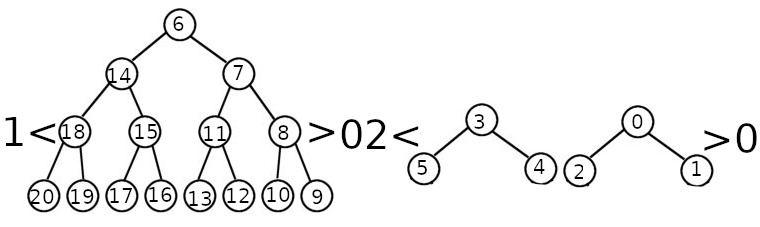
\includegraphics[width=\textwidth]{exemple_ral_entier.png}
\end{figure}
    
\end{frame}

\begin{frame}[fragile]{Skew RAL: lookup : $int$ $\rightarrow$ $'a$ RAL $\rightarrow$ $'a$}
\begin{lstlisting}
let lookup i st =
  let rec aux i st =
    match st with
    | [] -> raise (Failure "lookup")
    | (w, One (_, t)) :: ts ->
        if i < w then lookup_tree w i t else aux (i - w) ts
    | (w, Two (_, t1, t2)) :: ts ->
        if i < w then lookup_tree w i t2
        else aux (i - w) ((w, One (0, t1)) :: ts)
  in
  assert (is_well_formed st);
  aux i st
\end{lstlisting}
    
\end{frame}



\begin{frame}[fragile]{Skew RAL : lookup\_tree}
\begin{lstlisting}
let rec lookup_tree w i t =
  if i < 0 || i > w then raise (Failure "lookup_tree")
  else
    match (w, i, t) with
    | 1, 0, Leaf x -> x
    | _, 0, Node (x, _, _) -> x
    | w, i, Node (_, t1, t2) ->
        if i <= w / 2 then lookup_tree (w / 2) (i - 1) t2
        else lookup_tree (w / 2) (i - 1 - (w / 2)) t1
    | _ -> assert false
\end{lstlisting}
    
\end{frame}

\begin{frame}{Skew RAL : update}

En tous points similaire à lookup, seulement quand on arrive à la valeur cherchée, on la remplace au lieu de la renvoyer.
    
\end{frame}

\begin{frame}{Skew RAL : lookup}

Peut-on coder l'indice de lookup/update en skew bin ?
\phantom{Oui !}
    
\end{frame}

\begin{frame}{Skew RAL : lookup}

Peut-on coder l'indice de lookup/update en skew bin ?\\
Oui !\\
On s'affranchit des $int$ $OCaml$ et on travaille uniquement avec nos $Skew$ $Bin$ et nos $RAL$
    
\end{frame}

\begin{frame}{Skew RAL : lookup\_bin : $SBin$ $\rightarrow$ $'a$ RAL $\rightarrow$ $'a$}
\begin{figure}
    \centering
   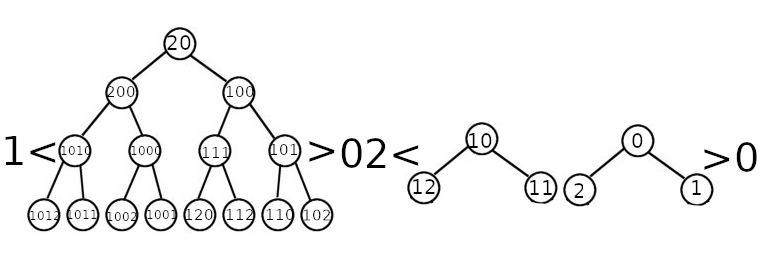
\includegraphics[width=\textwidth]{exemple_ral_sbin.png}
\end{figure}
On renverse nos argument pour avoir le bit de poids fort au début, et on transforme la distance "relative" en distance "absolue"\\
Il nous suffit d'avoir une méthode pour comparer deux RAL et le tour est joué !
\end{frame}

\begin{frame}[fragile]{Skew RAL : compare}
    \begin{lstlisting}
let rec compare b1 b2 =
  match (b1, b2) with
  | [], [] -> 0
  | [], _ -> -1
  | _, [] -> 1
  | (O, d) :: ts1, (O, d2) :: ts2 ->
      if d = d2 then compare ts1 ts2 else if d > d2 then 1 else -1
  | (T, d) :: ts1, (T, d2) :: ts2 ->
      if d = d2 then compare ts1 ts2 else if d > d2 then 1 else -1
  | (O, d) :: _, (T, d2) :: _ -> if d > d2 then 1 else -1
  | (T, d) :: _, (O, d2) :: _ -> if d >= d2 then 1 else -1
    \end{lstlisting}
\end{frame}

\begin{frame}[fragile]{Skew RAL : lookup\_up\_bin}
\begin{lstlisting}
let lookup_bin (i : skew) (st : 'a skew_tree) =
    match (i, st) with
    |... cas de base ...
    | (_, d1) :: _, (_, One (d2, t)) :: ((_, One (_, _)) :: _ as ts) ->
        if d1 <= d2 && compare i (to_bin ts) >= 0 then
          let tail = to_bin ts in
          lookup_tree_bin (sub_composed i tail) t
        else (
          assert (compare i (to_bin ts) < 0);
          aux i ts)
    ...
\end{lstlisting}
    
\end{frame}


    \begin{frame}[fragile]{Skew RAL : lookup\_up\_bin}
\begin{lstlisting}
    ...
    | (c, d1) :: _, (_, One (d2, t)) :: ((_, Two (d3, _, _)) :: [] as ts) ->
        if d1 <= d2 && if c = O then d1 > d3 else d1 >= d3 then (
          assert (compare i (to_bin ts) >= 0);
          (* car forme canonique donc 2 suivi par [] *)
          let tail = to_bin ts in
          lookup_tree_bin (sub_composed i tail) t)
        else (
          assert (if c = O then d1 <= d3 else d1 < d3);
          aux i ts)
\end{lstlisting}
    
\end{frame}

\begin{frame}{Skew RAL : lookup\_tree\_bin}
\begin{figure}
    \centering
   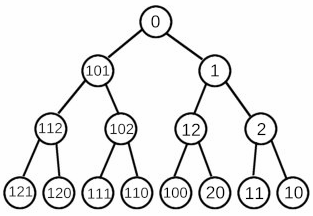
\includegraphics[width=\textwidth]{full_tree_numbered.png}
\end{figure}
    
\end{frame}

\begin{frame}[fragile]{Skew RAL : lookup\_tree\_bin}
\begin{lstlisting}
let rec lookup_tree_bin (i : skew) (t : 'a tree)
  match t with
  | Leaf a -> assert (i = []); a
  | Node (a, Leaf a2, Leaf a3) ->
      if i = [] then a
      else if i = [ (O, 0) ] then a3
      else if i = [ (T, 0) ] then a2
      else assert false
  | Node (a, t1, t2) ->
      if i = [] then a
      else
        let i_minus_one = sub_composed i [ (O, 0) ] in
        if compare i [ (O, height t - 1) ] > 0 then
          lookup_tree_bin (minus_one_msb i_minus_one) t1
        else lookup_tree_bin i_minus_one t2
\end{lstlisting}
    
\end{frame}

\begin{frame}{Et après ?}
\begin{itemize}
    \item SBin $\rightarrow$ forme canonique
    \item soustraction et somme
\end{itemize}
    
\end{frame}




\end{document}
